\documentclass{beamer}
\setbeamertemplate{navigation symbols}{}


\bibliographystyle{plain}

\usepackage{beamerthemeshadow}
\setbeamertemplate{caption}[numbered]

\hypersetup{colorlinks}

\def\gw#1{gravitational wave#1 (GW#1)\gdef\gw{GW}}
\def\gwb#1{gravitational wave burst#1 (GWB#1)\gdef\gw{GWB}}
\def\ns#1{neutron star#1 (NS#1)\gdef\ns{NS}}

\newcommand{\red}[1]{{\color{red}{#1}}}

\setbeamertemplate{bibliography item}[text]

\begin{document}
\title{}
\subtitle{Gravitational Wave Bursts: Inferences Without (Many) Assumptions}  
\author{James A. Clark}
%\institute{Georgia Institute Of Technology}
\date{} 

\begin{frame}[plain]
\titlepage
\end{frame}

\begin{frame}\frametitle{Table of contents}\tableofcontents
\end{frame} 

\section{Me}

\begin{frame}
    \frametitle{Background \& Interests}
    \begin{itemize}
        \item
    \end{itemize}
\end{frame}

\section{Gravitational Waves}

\begin{frame}
    \tableofcontents[currentsection]
\end{frame}


\subsection{Sources}
\begin{frame}
    \frametitle{Sources}
    \begin{itemize}
        \item \dots
    \end{itemize}
\end{frame}

\subsection{Data Analysis}
\begin{frame}
    \frametitle{Gravitational Wave ``Burst'' Analyses}
    \begin{itemize}
        \item \dots
    \end{itemize}
\end{frame}

\section{Past/Current Work}

\begin{frame}
    \tableofcontents[currentsection]
\end{frame}

\begin{frame}
    \frametitle{Gamma-ray Bursts}
    \begin{itemize}
        \item GRB\,051103~\cite{2012arXiv1201.4413T}
    \end{itemize}

    \begin{columns}[]
        \column{0.5\textwidth}
        \begin{center}
        \begin{figure}
            \vspace*{-0.5cm}
            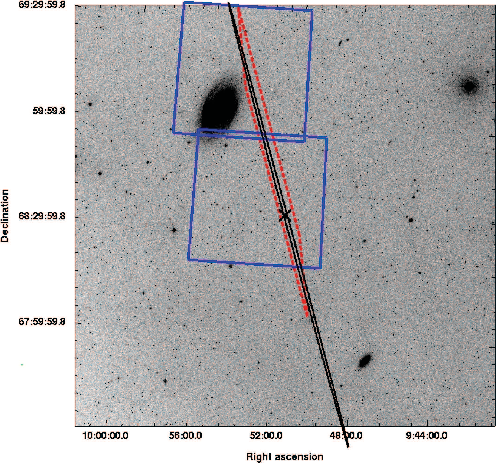
\includegraphics[scale=0.6]{m81_from_Hurley10.pdf} 
        \end{figure}
        \end{center}

        \column{0.5\textwidth}
        \begin{block}{Some text}
            Goes here
        \end{block}
    \end{columns}
\end{frame}

\begin{frame}
    \frametitle{Gamma-ray Bursts}

    \begin{itemize}
        \item GRB\,051103~\cite{2012arXiv1201.4413T}
    \end{itemize}

    \begin{columns}[]
        \column{0.5\textwidth}
        \begin{block}{Some text}
            Goes here
        \end{block}

        \column{0.5\textwidth}
        \begin{center}
        \begin{figure}
            \vspace*{-1.0cm}
            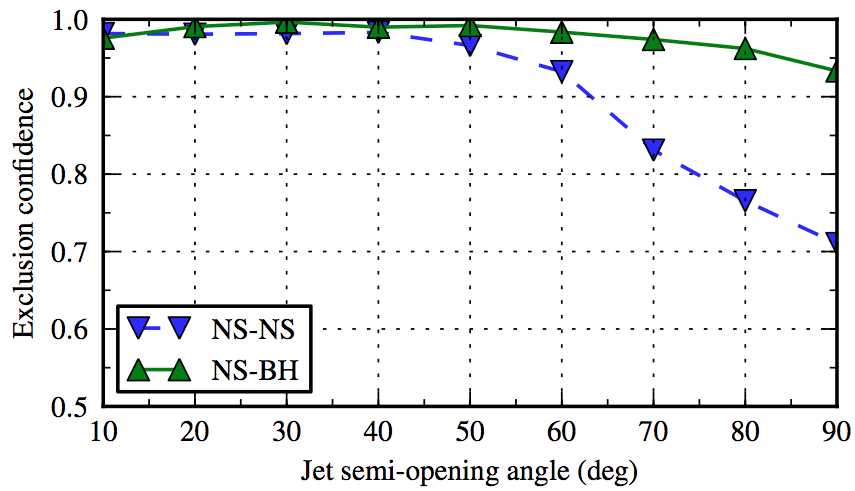
\includegraphics[scale=0.18]{jet_exc_PRODUCTION.png}  \\
            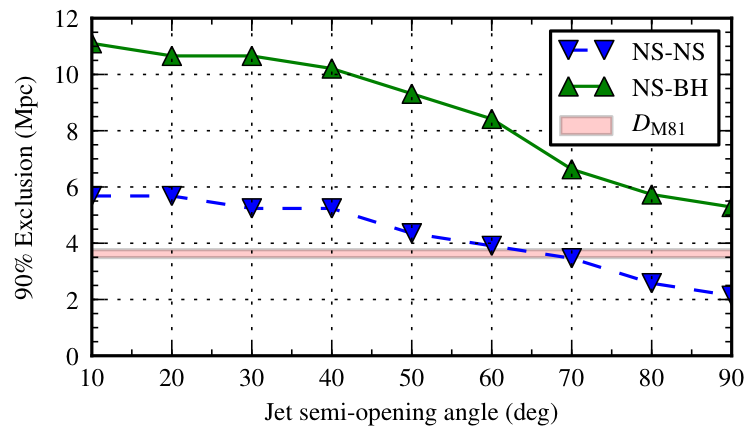
\includegraphics[scale=0.2]{D90_exc_PRODUCTION.png} 
        \end{figure}
        \end{center}
    \end{columns}

\end{frame}

\begin{frame}
    \frametitle{GWBs \& Binary Neutron Stars}
    \begin{itemize}
        \item
    \end{itemize}
\end{frame}

%\begin{frame}
%    \frametitle{\gwb{s} \& Isolated Neutron Stars}
%    \begin{itemize}
%        \item
%    \end{itemize}
%\end{frame}

\begin{frame}
    \frametitle{Binary Black Holes}
    \begin{itemize}
        \item
    \end{itemize}
\end{frame}

\section{Future GW Astronomy}

\begin{frame}
    \tableofcontents[currentsection]
\end{frame}

\subsection{When will we see something, what will we see?}

\begin{frame}
    \frametitle{Advanced LIGO}
    When will we see something?
    \begin{itemize}
        \item
    \end{itemize}
\end{frame}

\section{Conclusion}

\begin{frame}
    \frametitle{Summary}
\end{frame}

\begin{frame}
    \frametitle{References}
    \bibliography{biblio}
\end{frame}



\end{document}
